\section{Related Work}

\subsection{Facial Retargetting and Enactment}
Recent advances in capture technology such as ~\cite{cao2015real,f2f,laine2016facial} have been able to capture faces with high-fidelity using only monocular input. 
~\cite{olszewski2016high} uses a head-mounted rig and a mouth-camera to regress model PCA expression coefficients for high-fidelity speech animation.  

~\cite{f2f} reenacts a video sequence by using multiple frames of the target video sequence to construct a geometric identity of the target. 
Similarly, ~\cite{rewrite} adopts a multi-scale approach to replace a face from one video sequence with the appearance from a different video sequence. 
The limitation here is that the animated face's identity is fixed - the system cannot puppeteer an arbitrary person from an image. To address this issue, ~\cite{replace} switches the appearance of one person's face onto another in a realistic fashion. In ~\cite{malleson2015facedirector}, the authors compute a nonlinear temporal synchronization between two videos of the same actor that can be blended for a novel performance. The work of ~\cite{garrido2014automatic} can replace the face of the actor in a target video with the face of a source video. The authors of ~\cite{garrido2013reconstructing} are able to reconstruct detailed 3D facial geometry from a monocular video.  
However, all these methods require a video of the target in order to do photorealistic facial retargetting, rather than using only a single target image as in our method.

~\cite{spacey} learns a controllable model of a face from an image collection that can be puppeteered.  Though it does not require video, it does require many different images to work.  ~\cite{face-swap} uses a deep network to swap faces between two images.

\subsection{Capturing and Retargeting Photorealistic Mouth Interior}
Capturing and modeling the mouth region has always been a challenge. Existing works include ~\cite{Chuang:2005:MSE,Wampler:2007:DES,Taylor:2012:DUV,FanWSX15,edwardsjali}, which use audio input to render the mouth region. \cite{wu2016model} fits a 3D model to reconstruct a teeth model from a photograph as input. 
\cite{garrido2015vdub} and \cite{thies2015real} improve the photorealism of their 3D teeth models with 3D textured teeth proxies.
These works are not well suited for photo-realistic teeth retargeting because they only track the mouth of the source image and do not consider a target image at all.
%Other works such as ~\cite{vlasic2005face} and~\cite{replace} copy the mouth directly from the source mouth region.
 In their recent work,~\cite{f2f} fills in the inner mouth region by searching for similar mouth frames in a target video.  
In contrast with previous work, we do not need a target video to infer photo-realistic teeth texture. 
Instead, we only need a single RGB image of the target image that does not necessarily contain teeth and use a conditional GAN to infer contents in the mouth which are further upsampled and refined by flowing the pixels from the source video.   

\begin{figure*}[t]
	\centering
	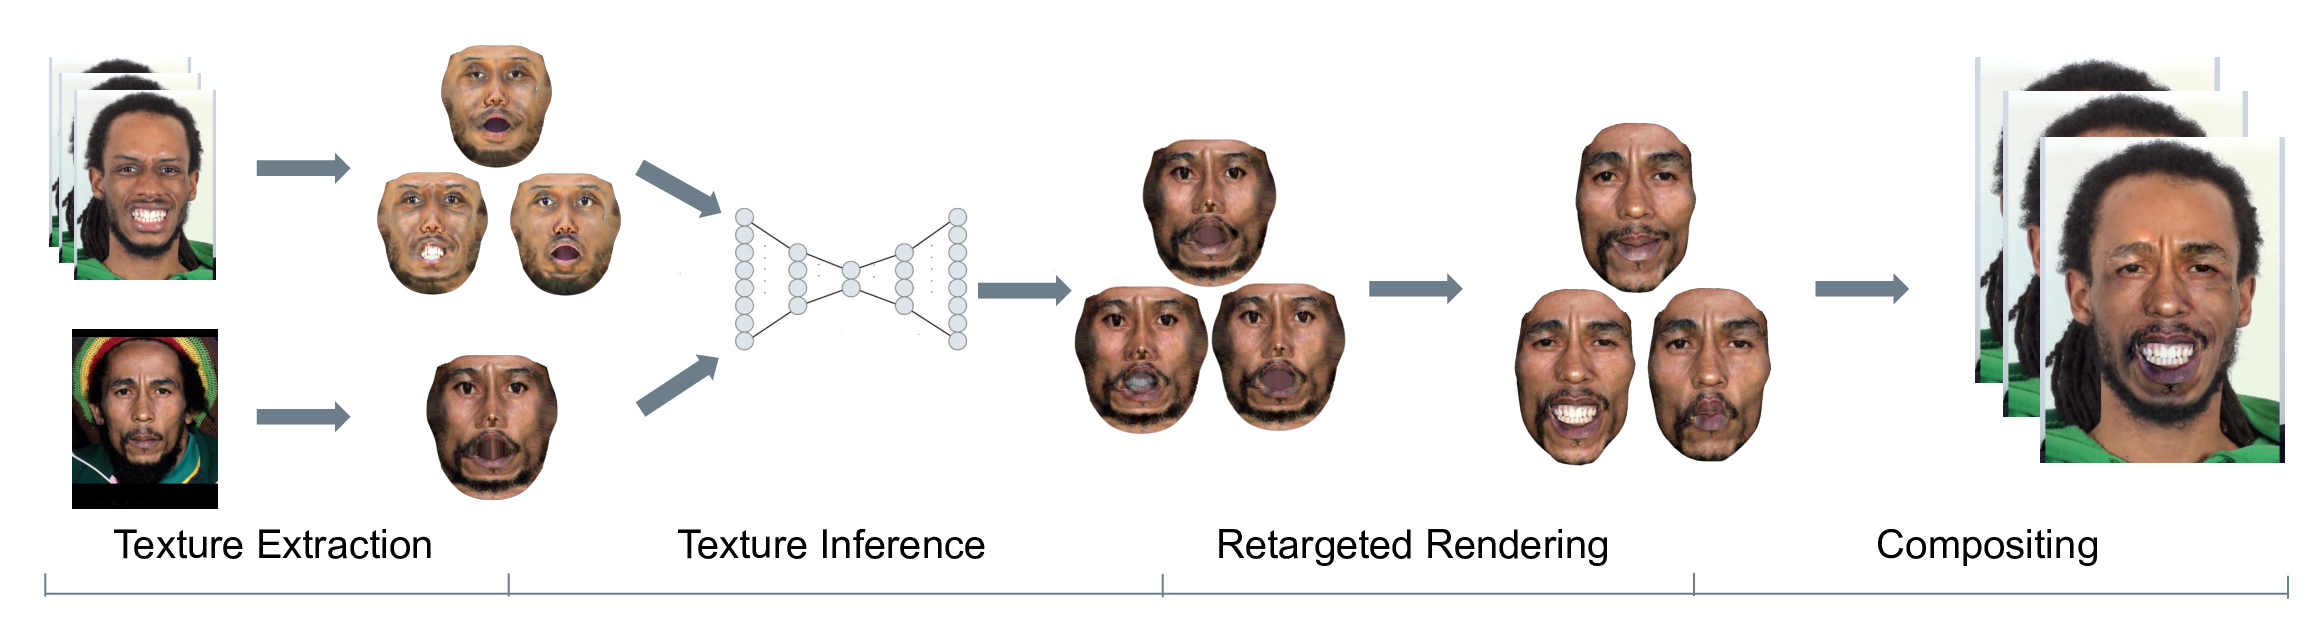
\includegraphics[width=1\linewidth]{figures/overview/pipeline_new2.png}
	\caption{Overview of the pipeline.}\label{fig:arch_content}
	\vspace{-0.15in}
\end{figure*}


\subsection{Deep Generative Model for Texture Synthesis}

The rise of deep learning has brought many advances in image synthesis. Generative Adversarial Models \cite{gan} have proved especially capable of generating sharp and realistic images. 
More specifically, we use a conditional GAN~\cite{cgan} to enable end-to-end synthesis of high-resolution facial textures conditioned on the target identity and source facial expressions. While conditional GANs have been used for a wide range of applications such as image-to-image translation \cite{pix2pix}, face image generation \cite{gauthier2014}, image inpainting \cite{pathak2016context, yang2016high}, and style transfer \cite{li2016precomputed}, to our knowledge conditional generative adversarial models have never been used for the purpose of generating high-detailed textures.

Previous facial synthesis works that do not use conditional GANs include  \cite{liu2007face}, which hallucinates high-resolution faces from low-resolution images using a local patch-based Markov network, and
\cite{mohammed2009visio}, which generates novel face images by learning a probabilistic model from a set of training faces. 
However, neither of these results are realistic and artifact-free in high-resolution. \cite{golovinskiy2006statistical} uses statistical models to generate wrinkles and pores on facial geometry, but cannot do so for textures. \cite{saito2016} uses a deep learning framework to generate high resolution textures from a single image, but they cannot infer details like wrinkles and the inner mouth region on their textures for different expressions as we can.
